%%% Uncomment only one of the next two lines (depending on whether you want the answers printed)
\documentclass[answers,fleqn,addpoints,12pt]{exam}

% \usepackage[usenames, dvipsnames]{color} % defines a new color

\renewcommand{\solutiontitle}{\noindent\textbf{Answer: }}
%% How to print correct answer choices:
\CorrectChoiceEmphasis{\itshape\bfseries} %% <-- bold italics
\newcommand\coursename{DS 644}
\newcommand\semester{Spring 2023}

% \pointsinmargin
\pointpoints{pt}{pts}
% \marginpointname{pts}
% \marginbonuspointname{pts}

\makeatletter
\newif\ifanswers
\@ifclasswith{exam}{answers}{\answerstrue}{\answersfalse}
\makeatother
\newcommand{\scratchpage}{%
  \ifanswers % do nothing
  \else \newpage \thispagestyle{empty} \begin{center} -- scratch -- \end{center} \fi}

%% Change geometry if you want:
\usepackage[top=1cm, left=2cm,right=2cm,bottom=1cm]{geometry}%

\usepackage{amsmath}
\usepackage{amsthm,amssymb}
\usepackage{mathtools}
\usepackage{comment}
\usepackage{unixode}
\newtheorem*{answer}{{\bf Answer}}
\newtheorem*{answers}{{\bf Answers}}
\newtheorem*{explanation}{{\bf Explanation}}

% Create a True False question format
\newcommand*{\TrueFalse}[1]{%
\ifprintanswers
    \ifthenelse{\equal{#1}{T}}{%
        \textbf{TRUE}\hspace*{14pt}False
    }{
        True\hspace*{14pt}\textbf{FALSE}
    }
\else
    {True}\hspace*{20pt}False
\fi
} 
%% The following code is based on an answer by Gonzalo Medina
%% http://tex.stackexchange.com/a/13106/39194
\newlength\TFlengthA
\newlength\TFlengthB
\settowidth\TFlengthA{\hspace*{1.16in}}
\newcommand\TFQuestion[2]{%
    \setlength\TFlengthB{\linewidth}
    \addtolength\TFlengthB{-\TFlengthA}
    \parbox[t]{\TFlengthB}{#2}
    \parbox[t]{\TFlengthA}{\TrueFalse{#1}}}



%% Some of my own personal favoriate macros... (remove these if you want)
\renewcommand{\vec}[1]{\mathbf{#1}}
%% To make a boldface vector, use backslash v in front of the 
%% letter and add a new command for that letter here or in 
%% the macros.tex file:
\newcommand\im{\ensuremath{\operatorname{im}}}
\newcommand\rank{\ensuremath{\operatorname{rank}}}
\newcommand\nullity{\ensuremath{\operatorname{nullity}}}
\newcommand{\join}{\ensuremath{\vee}}
\newcommand{\meet}{\ensuremath{\wedge}}
\newcommand{\Z}{\ensuremath{\mathbb{Z}}}
\newcommand{\<}{\ensuremath{\langle}}
\renewcommand{\>}{\ensuremath{\rangle}}
\newcommand\vR{\ensuremath{\operatorname{R}}}
\newcommand\vN{\ensuremath{\operatorname{N}}}
\newcommand\vC{\ensuremath{\operatorname{C}}}
\newcommand\va{\vec{a}}
\newcommand\vb{\vec{b}}
\newcommand\ve{\vec{e}}
\newcommand\vE{\vec{E}}
\newcommand\vu{\vec{u}}
\newcommand\vv{\vec{v}}
\newcommand\vw{\vec{w}}
\newcommand\vs{\vec{s}}
\newcommand\vx{\vec{x}}
\newcommand\vy{\vec{y}}
\newcommand\vz{\vec{z}}
\newcommand\vzero{\vec{0}}
\newcommand{\probskip}{\vskip1.5cm}
\newcommand{\finans}[1]{\ensuremath{\underline{\underline{#1}}}}
\newcommand{\dotsize}{1pt}
\newcommand{\Heq}{\ensuremath{ \; \stackrel{\mathrm{H}}{=}} \; }

\pagestyle{foot}
%%% Running footer will have a space for page score (if this is not the solution key)
\ifanswers  %% do nothing
\else
\runningfooter{}{}{Score for this page: \makebox[1in]{\hrulefill} out of \pointsonpage{\thepage}}
\fi



\newcommand{\figscl}{.5}
\newcommand{\tf}[1][{}]{%
  \fillin[#1][0.25in]%
}

\newcommand\explain[1]{%
  \ifanswers
  \begin{EnvUplevel}
    {\small \underline{Explanation}. #1} 
  \end{EnvUplevel}
  \else \fi}

\ifanswers
\usepackage{background}
\backgroundsetup{
  color=black,
  opacity=.25,
  scale=2,
  contents={\textsc{FOR PERSONAL USE ONLY -- DO NOT DISTRIBUTE}}%
}
\fi

\newcommand\myheader{%
  \noindent {\bf \coursename : \semester}\hfill \ifanswers {\bf ANSWERS} \hfill {\bf \assignment} 
  \else {\bf \assignment \hfill Due \duedate 11:59pm}
  \\[5mm]
  Name: \underline{\phantom{XXXXXXXXXXXXXXXXXXXX}} \hfill Student ID: \underline{\phantom{XXXXXXXXXXXX}}
  \fi%
}
\checkboxchar{$\Box$}% \renewcommand{\questionshook}{%


\begin{document}


\noindent {\bf \coursename : \semester}\hfill 
{\bf Midterm Examination} \hfill \ifanswers {\bf ANSWERS}
\else

\begin{center}
  \fbox{\fbox{\parbox{7in}{\centering
        {\bf RULES}
        \begin{itemize}
        \item {\bf No books}, {\bf no notes}, and {\bf no calculators}.
        \item {\bf No bathroom breaks} until after you have completed and submitted the exam.
        \item {\bf All phones must be completely silent} for the duration of the exam, so please \\
          {\it turn off your phone now!}
        \end{itemize}}}}
\end{center}
\vspace{0.2in}

\noindent    {\it Cheating will not be tolerated.}  If there is any indication that a
student may have given or received unauthorized aid on this test, the case 
will be referred to the Office of the Dean of Students.
When you finish the exam, you must sign the following pledge:\\
\\\\
``On my honor as a student I,
\underline{\phantom{XXXXXXXXXXXXXXXXXXXXXX}}, have neither
given nor received unauthorized aid on this exam.''
\hbox{} \hskip .25cm {\small (print name clearly)}\\
\\\\
\vspace{0.1in}
\makebox[\textwidth]{Signature:\enspace\hrulefill ~Date: 
\underline{\phantom{x} 27 March 2023 \phantom{x}}}

\vskip2cm

{\small \begin{center} \gradetable[h][pages] \end{center} }

~
\newpage
\fi

\pagestyle{foot}

% \thispagestyle{fancy}

\noindent \textbf{Instructions}. Answer the following multiple choice questions by selecting all correct choices.
If a question has more than one correct choice, it will say in parentheses how many items you should select.
\textit{Select all correct choices to receive full credit!}

%%% HOMEWORK 1 %%%

\begin{questions} % Begins the questions environment

  % Question 1
  \question[6] \textbf{Programming Paradigms}
  \begin{parts}
    \part Which of the following is {\it not} an example of a programming paradigm?

    \begin{oneparcheckboxes}
      \choice Declarative
      \choice Functional
      \CorrectChoice Immutable
      \choice Imperative
      \choice Object-oriented
    \end{oneparcheckboxes}

    \medskip

    \part Which of the following characteristics are typical of imperative programs? (select two)

    \begin{checkboxes}
      \choice Values of variables do not change or ``mutate'' (they are \textit{immutable}).
      \CorrectChoice Iteration is typically performed with \texttt{for} or \texttt{do-while} loops.
      \choice Iteration is typically performed with recursion.
      \CorrectChoice Functions often have \textit{side-effects}.
    \end{checkboxes}

    \smallskip

    \part Which of the following characteristics are typical of functional programs?  (select two)
    \begin{checkboxes}
      \CorrectChoice Values of variables do not change or ``mutate'' (they are \textit{immutable}).
      \choice Iteration Is typically performed with \texttt{for} or \texttt{do-while} loops.
      \CorrectChoice Iteration is typically performed with recursion.
      \choice Functions often have \textit{side-effects}.
    \end{checkboxes}
  \end{parts}

\vskip1cm

  % Question 2
  \question[2] A \textit{higher-order function} is a function that
  \begin{checkboxes}
    \choice can be passed as an argument to other functions.
    \choice can be returned as output by other functions.
    \choice can be called a higher order of times than ordinary functions.
    \CorrectChoice accepts another function as input.
    \choice takes a long time to compute (i.e., has higher order time complexity).
  \end{checkboxes}

\vskip1cm
\begin{comment}


  % Question 3
  \question[3] An expression \texttt{e} is called \textit{referentially transparent} provided
  \begin{checkboxes}
    \choice the value of \texttt{e}, when it is reduced to ``normal form,'' is obvious or ``transparent.''
    \choice the values all expressions to which \texttt{e} refers are obvious or ``transparent.''
    \CorrectChoice for all programs \texttt{p}, all occurrences of \texttt{e} in \texttt{p} can be replaced by the result of evaluating \texttt{e} without affecting the meaning of \texttt{p}.
    \choice none of the above
  \end{checkboxes}

\end{comment}


  % Question 3
  \question[2]
 Which \textit{two} of the following terms are used to describe the programming paradigm of Scala?

    \begin{oneparcheckboxes}
      \choice assembly
      \choice declarative
      \CorrectChoice functional
      \choice imperative
      \CorrectChoice object-oriented
    \end{oneparcheckboxes}

    \medskip

  \question[3]
 What is the result of the following program?
    \begin{verbatim}
    val x = 2
    def f(y: Int) = y * y
    val result = {
      val x = f(2)
      x * x
    } + x
    \end{verbatim}
    \begin{oneparcheckboxes}
      \choice 6
      \choice 16
      \CorrectChoice 18
      \choice  32
      \choice None---it does not terminate.
    \end{oneparcheckboxes}

    \newpage


 \question[3]
%   \begin{parts}
%     \part Which of the functions shown in the figure is tail-recursive?

%     \begin{oneparcheckboxes}
%       \choice \texttt{funone}
%       \choice \texttt{funtwo}
%       \CorrectChoice \texttt{funthree}
%       \choice  \texttt{funfour}
%       \choice none of these
%     \end{oneparcheckboxes}

% \vskip2cm

   Why do you think the designers of Scala thought it was important to support ``tail-recursive'' functions?

    \begin{checkboxes}
      \choice Because recursion should be carried out on the tail, not the head.
      \choice Because recursion should be carried out on the head, not the tail.
      \CorrectChoice Because they are ``stack-safe''---they help us avoid stack overflows.
      \choice Because they are ``disk-safe''---they help us avoid network storage leaks.
    \end{checkboxes}


\begin{comment}
\vskip1cm

  % Question 5
  \question[6] Consider the following code.

  \begin{verbatim}
    def sq(x: Double): Option[Double] =
      if (x < 0) None
      else Some(Math.sqrt(x))

    val list = List(-1.0, 4.0, 9.0)
  \end{verbatim}

  \begin{parts}
    \part To what does the expression \texttt{list.map(sq)} evaluate?

    \begin{checkboxes}
      \choice \texttt{List(2.0, 3.0)}
      \CorrectChoice \texttt{List(None, Some(2.0), Some(3.0))}
      \choice \texttt{Some(List(2.0, 3.0))}
      \choice \texttt{None}
      \choice none of the above
    \end{checkboxes}


\part To what does the expression \texttt{list.flatMap(sq)} evaluate?

    \begin{checkboxes}
      \CorrectChoice \texttt{List(2.0, 3.0)}
      \choice \texttt{List(None, Some(2.0), Some(3.0))}
      \choice \texttt{Some(List(i, 2.0, 3.0))}
      \choice \texttt{None}
      \choice none of the above
    \end{checkboxes}
  \end{parts}
\end{comment}

\medskip

\question[12] The parts below refer to the function\\[8pt]
  \texttt{def test(x:Bool, y:Int) = if (x) (y + 2)/y else 0}\\[6pt]
  Let CBN = call-by-name\\[6pt]
  and CBV = call-by-value.

  %where \texttt{loop()} is an infinite (non-terminating) loop.
\medskip

  \begin{parts}
    \part Which strategy evaluates \texttt{test(true, 2)} most efficiently (in the fewest steps)?

    \begin{oneparcheckboxes}
      \choice CBN % is more efficient
      \choice CBV % is more efficient
      \CorrectChoice CBN and CBV require the same number of steps
      %\choice the program does not terminate
    \end{oneparcheckboxes}

    \explain{They both perform one addition (\texttt{2 + 2}) and one division (\texttt{4/2}).}

    \bigskip

    \part Which strategy evaluates \texttt{test(true, 1+1)} most efficiently?

    \begin{oneparcheckboxes}
      \choice CBN %is  more efficient
      \CorrectChoice CBV %is more efficient
      \choice CBN and CBV require the same number of steps
      %\choice the program does not terminate
    \end{oneparcheckboxes}

    \explain{CBV performs two additions (\texttt{1 + 1} and \texttt{2 + 2}) and one division (\texttt{4/2}), while CBN performs three additions (\texttt{1 + 1} and \texttt{2 + 2} and \texttt{1 + 1} again) and one division (\texttt{4/2}).}

    \bigskip

    \part Which strategy evaluates \texttt{test(false, 2)} most efficiently?

    \begin{oneparcheckboxes}
      \choice CBV %is more efficient
      \choice CBN %is more efficient
      \CorrectChoice CBN and CBV require the same number of steps
      %\choice the program does not terminate
    \end{oneparcheckboxes}


    \bigskip

    \part Which strategy evaluates \texttt{test(false, 1+1)} most efficiently?

    \begin{oneparcheckboxes}
      \CorrectChoice CBN %is more efficient
      \choice CBV %is more efficient
      \choice CBN and CBV require the same number of steps
      %\choice the program does not terminate
    \end{oneparcheckboxes}

    \explain{CBV performs one addition (\texttt{1 + 1}), while CBN performs no operations.}

  \end{parts}

\begin{comment}
  % Question 6
  \question[12] The parts below refer to the function \texttt{test(x:Int, y:Int) = x * x}.

  \begin{parts}
    % \part For the function call \texttt{test(2, 3)}, which evaluation strategy is  most efficient (takes the least number of steps)?

    % \begin{checkboxes}
    %   \choice call-by-value is more efficient
    %   \choice call-by-name is more efficient
    %   \CorrectChoice call-by-value and call-by-name require the same number of steps
    %   \choice the program does not terminate
    % \end{checkboxes}

    % \explain{In both cases we have to do one multiplication (\texttt{2 * 2}).}

    \part For the function call \texttt{test(3 + 4, 8)}, which evaluation strategy is most efficient?

    \begin{checkboxes}
      \CorrectChoice call-by-value is more efficient
      \choice call-by-name is  more efficient
      \choice call-by-value and call-by-name require the same number of steps
      \choice the program does not terminate
    \end{checkboxes}

    \explain{Call-by-value performs one addition (\texttt{3 + 4}) and one multiplication (\texttt{7 * 7}), whereas
      call-by-name performs two additions and one multiplication (\texttt{(3 + 4) * (3 + 4)}).}

    \part For the function call \texttt{test(7, 2*4)}, which evaluation strategy is most efficient?

    \begin{checkboxes}
      \choice call-by-value is more efficient
      \CorrectChoice call-by-name is more efficient
      \choice call-by-value and call-by-name require the same number of steps
      \choice the program does not terminate
    \end{checkboxes}

    \explain{Call-by-value performs two multiplications (\texttt{2 * 4} and \texttt{7 * 7}), whereas
      call-by-name performs just one multiplication (\texttt{7 * 7}).}

    \part For the function call \texttt{test(3+4, 2*4)} which evaluation strategy is most efficient?

    \begin{checkboxes}
      \choice call-by-value is more efficient
      \choice call-by-name is more efficient
      \CorrectChoice call-by-value and call-by-name require the same number of steps
      \choice the program does not terminate
    \end{checkboxes}

    \explain{Call-by-value performs one addition (\texttt{3 + 4}) and two multiplications (\texttt{2 * 4} and \texttt{7 * 7}), and
      call-by-name performs two additions and one multiplication (\texttt{(3 + 4) * (3 + 4)}).}

  \end{parts}
\end{comment}
  \medskip

  %%% HOMEWORK 2 %%%

  % Question 1
  \question[12] \textbf{Higher-order Functions}

All parts of this question refer to the following \texttt{sum} function.

\begin{verbatim}
def sum(f: Int => Int): (Int, Int) => Int = {
  def sumF(a: Int, b: Int): Int = {
    if (a > b) 0
    else f(a) + sumF(a + 1, b)
  }
  sumF
}
\end{verbatim}

\begin{parts}
  \part What does \texttt{sum(2, 3)} compute?

    \begin{checkboxes}
      \choice \texttt{2 + 3}
      \choice  \texttt{2 + 2 + 3 + 3}
      \choice  \texttt{2 * 2 + 3 * 3}
      \choice  a function that takes two integer arguments and returns their sum
      \choice  \texttt{sum(2, 3)} causes a run-time error.
      \CorrectChoice \texttt{sum(2, 3)} causes a compile-time error.
    \end{checkboxes}

\newpage

    \part What does \texttt{sum(x => x)(2, 3)} compute?

    \begin{checkboxes}
      \CorrectChoice \texttt{2 + 3}
      \choice \texttt{2 + 2 + 3 + 3}
      \choice \texttt{2 * 2 + 3 * 3}
      \choice a function that takes two integer arguments and returns their sum
      \choice \texttt{sum(x => x)(2, 3)} causes a run-time error.
      \choice \texttt{sum(x => x)(2, 3)} causes a compile-time error.
    \end{checkboxes}

\medskip
\part What does \texttt{sum(x => x)} return?

\begin{checkboxes}
  \choice \texttt{2 + 3}
  \choice \texttt{2 + 2 + 3 + 3}
  \choice \texttt{2 * 2 + 3 * 3}
  \CorrectChoice a function that takes two integer arguments and returns their sum
  \choice \texttt{sum(x => x)(2, 3)} causes a run-time error.
  \choice \texttt{sum(x => x)(2, 3)} causes a compile-time error.
\end{checkboxes}

\medskip
\part What does \texttt{sum(x => x + x)(2, 3)} compute?

\begin{checkboxes}
\choice \texttt{2 + 3}
\CorrectChoice \texttt{2 + 2 + 3 + 3}
\choice \texttt{2 * 2 + 3 * 3}
\choice a function that takes two integer arguments and returns their sum
\choice \texttt{sum(x => x + x)(2, 3)} causes a run-time error.
\choice \texttt{sum(x => x + x)(2, 3)} causes a compile-time error.
\end{checkboxes}

\medskip
\part What does \texttt{sum(x => x * x)(2, 3)} compute?

\begin{checkboxes}
\choice \texttt{2 + 3}
\choice \texttt{2 + 2 + 3 + 3}
\CorrectChoice \texttt{2 * 2 + 3 * 3}
\choice a function that takes two integer arguments and returns their sum
\choice \texttt{sum(x => x * x)(2, 3)} causes a run-time error.
\choice \texttt{sum(x => x * x)(2, 3)} causes a compile-time error.
\end{checkboxes}

\medskip
\part What does \texttt{sum(x => x / 1.0)(2, 3)} compute?

\begin{checkboxes}
\choice \texttt{2 + 3}
\choice \texttt{2 + 2 + 3 + 3}
\choice \texttt{2 * 2 + 3 * 3}
\choice a function that takes two integer arguments and returns their sum
\choice \texttt{sum(x => x/1.0)(2, 3)} causes a run-time error.
\CorrectChoice \texttt{sum(x => x/1.0)(2, 3)} causes a compile-time error.
\end{checkboxes}
\end{parts}

\newpage


\question[3] % \textbf{Scala Pattern Matching}

Consider the general form of pattern matching in Scala,

\begin{verbatim}
e match { case p1 => e1 ... case pn => en }
\end{verbatim}

Which of the following are true statements?

\begin{checkboxes}
\choice Scala matches the value of the selector \texttt{e} with the patterns \texttt{p1, ..., pn} in the order in which they are written.
\choice The match expression is rewritten to the right-hand side of the first case where the pattern matches the selector \texttt{e}.
\choice References to pattern variables are replaced by the corresponding parts in the selector.
\CorrectChoice All of the above.
\choice None of the above.
\end{checkboxes}

\medskip

\question[3] Consider the following Scala program.

\begin{verbatim}
trait Expr
case class Number(n: Int) extends Expr
case class Sum(e1: Expr, e2: Expr) extends Expr

object Number{ def apply(n: Int) = new Number(n) }

object Sum{ def apply(e1: Expr, e2: Expr) = new Sum(e1, e2) }

def eval(e: Expr): Int = e match {
  case Number(n) => n
  case Sum(e1, e2) => eval(e1) + eval(e2)
}
\end{verbatim}

What is the result of the following expression?

\begin{verbatim}
eval(Sum(Number(1), Number(2)))
\end{verbatim}

\begin{oneparcheckboxes}
\choice 0
\choice 1
\choice 2
\CorrectChoice 3
\choice None of the above.
\end{oneparcheckboxes}

\newpage

  % Q.2.5
  \question[6]
  %% def sq(x: Double): Option[Double] =
  %% if (x < 0) None
  %% else Some(Math.sqrt(x))
Let \texttt{val X = List(1, 2, 3)}\\
\phantom{(6 pts)} and \texttt{val Y = List(1, 2, 3)}.

\bigskip

  \begin{parts}
    \part To what does the expression \texttt{X.map(x => Y.map(y => y - x)))} evaluate?

    \medskip
    \begin{checkboxes}
      \choice \texttt{List(0, 0, 0, 0, 0, 0, 0, 0, 0)}
      \choice \texttt{List(List(0, 0, 0), List(0, 0, 0), List(0, 0, 0))}
      \choice \texttt{List(0, -1, -2, 1, 0, -1, 2, 1, 0)}
      \choice \texttt{List(0, 1, 2, -1, 0, 1, -2, -1, 0)}
      \CorrectChoice \texttt{List(List(0, 1, 2), List(-1, 0, 1), List(-2, -1, 0))}
    \end{checkboxes}

\bigskip
    \part To what does the expression \texttt{X.flatMap(x => Y.map(y => y - x)))} evaluate?

    \medskip
    \begin{checkboxes}
      \choice \texttt{List(0, 0, 0, 0, 0, 0, 0, 0, 0)}
      \choice \texttt{List(List(0, 0, 0), List(0, 0, 0), List(0, 0, 0))}
      \choice \texttt{List(List(0, -1, -2), List(1, 0, -1), List(2, 1, 0))}
      \CorrectChoice \texttt{List(0, 1, 2, -1, 0, 1, -2, -1, 0)}
      \choice \texttt{List(List(0, 1, 2), List(-1, 0, 1), List(-2, -1, 0))}
    \end{checkboxes}

  \end{parts}



\begin{comment}

\question Consider the Scala code below.

\begin{verbatim}
val x = List(1,2,3)
val y = List(0, x, 4)
\end{verbatim}


\begin{parts}


\part What is the type of \texttt{x}?

\begin{checkboxes}
\choice \texttt{List[T]}
\CorrectChoice \texttt{List[Int]}
\choice \texttt{List[Any]}
\choice \texttt{List[Nothing]}
\choice \texttt{List[Object]}
\end{checkboxes}

\part What is the type of \texttt{y}?

\begin{checkboxes}
\choice \texttt{List[T]}
\choice \texttt{List[Int]}
\CorrectChoice \texttt{List[Any]}
\choice \texttt{List[Nothing]}
\choice \texttt{List(0, x, 4)} causes a run-time error.
\choice \texttt{List(0, x, 4)} causes a compile-time error.
\end{checkboxes}

\part What is \texttt{y.length}?

\begin{checkboxes}
\choice 0
\CorrectChoice 3
\choice 5
\choice \texttt{y.length} causes a run-time error.
\choice \texttt{y.length} causes a compile-time error.
\end{checkboxes}

\part What is \texttt{x == List(1, 2, y.length)}?

\begin{checkboxes}
\choice \texttt{List(1, 2, 3)}
\choice \texttt{List(x, 1, 2, 3)}
\CorrectChoice \texttt{true}
\choice \texttt{false}
\choice None of these.
\end{checkboxes}
\end{parts}
\end{comment}

\bigskip

\question[9] Reducing lists with \texttt{foldLeft}.

Suppose you want to implement a (polymorphic) \texttt{reverse} function, which reverses the order of a given list, \texttt{xs: List[T]}, using Scala's \texttt{foldLeft} function.

You start with

\begin{verbatim}
def reverse[T](xs: List[T]): List[T] = (xs foldLeft ???)((ys, y) => ???)
\end{verbatim}

\begin{parts}

\part What aspect of the code above tells you that this \texttt{reverse} function will be {\it polymorphic}?

\begin{checkboxes}
\choice It operates on lists.
\choice The second \texttt{???} will be a function, so it's "higher-order."
\choice There is a folding or "reduction" operation involved.
\choice It is recursive.
\CorrectChoice It takes a type parameter \texttt{T}.
\end{checkboxes}

\part The first set of three question marks \texttt{???} should be replaced with which of the following?

\begin{oneparcheckboxes}
\choice \texttt{Nil}
\CorrectChoice \texttt{List[T]()}
\choice \texttt{List[T](0)}
\choice \texttt{ys :: y}
\choice \texttt{y :: ys}
\end{oneparcheckboxes}

\part The second set of three question marks \texttt{???} should be replaced with which of the following?

\begin{oneparcheckboxes}
\choice \texttt{Nil}
\choice \texttt{List[T]()}
\choice \texttt{List[T](0)}
\choice \texttt{ys :: y}
\CorrectChoice \texttt{y :: ys}
\end{oneparcheckboxes}
\end{parts}


\newpage


%%% HOMEWORK 3 %%%


\begin{comment}
\question[6] % \textbf{Principles of (functional) programming}


\begin{parts}
\part Which of the following are programming paradigms? (Select three.)

\begin{oneparcheckboxes}
\CorrectChoice Declarative
\CorrectChoice Functional
\choice Hadoop
\CorrectChoice Imperative
\choice Scala
\end{oneparcheckboxes}

\part What three concepts characterize a purely functional programming language?

\begin{oneparcheckboxes}
  \CorrectChoice referential transparency
\choice input/output
\CorrectChoice no side effects
\choice procedural
\CorrectChoice immutability
\end{oneparcheckboxes}
\end{parts}
\end{comment}

\begin{comment}

\question \textbf{Big data properties}.

  \begin{parts}
    \part In lecture we discussed the meaning of the term ``Big Data.'' We decided that, for simplicity, we will call data ``big'' when it is

    \begin{checkboxes}
    \choice at least 1Gb
    \CorrectChoice too big to fit in fast memory (cpu cache + ram) on a single compute node
    \choice too big to fit in all computer memory (whether fast or slow)
    \choice too big to be dealt with by traditional data-processing software
    \end{checkboxes}

\explain{We agreed that a good definition of ``Big Data'' for our purposes is data that is too large to fit in the fast computer memory of a single machine.  Although Wikipedia has an alternative definition---data that is ``too big to be dealt with by traditional data-processing application software''---and while that definition is not wrong, it is not the definition we agreed upon in this class.}

    \part ``Big Data'' concerns which of the following types of data?

\begin{oneparcheckboxes}
\choice structured
\choice semi-structured
\choice unstructured
\CorrectChoice all of these
\end{oneparcheckboxes}

\explain{Big Data is a blanket term for the data that are too large in size and complex in nature, and which may be structured, unstructured, or semi-structured, and may also be arriving at high velocity.}

\part JSON and XML are examples of which type of data?

\begin{oneparcheckboxes}
\choice structured
\choice unstructured
\CorrectChoice semi-structured
\choice none of these
\end{oneparcheckboxes}

\explain{Semi-structured data are that which have a structure but do not fit into the relational database. Semi-structured data are organized, which makes it easier for analysis when compared to unstructured data. JSON and XML are examples of semi-structured data.}

\part Which two of the following statements are true of unstructured data?

\begin{checkboxes}
\choice It is generally easier to analyze than other types of data.
\CorrectChoice It is often referred to as ``messy'' data.
\choice It fits neatly into a schema.
\CorrectChoice It is the most widespread type of data.
\choice It is usually found in tables.
\end{checkboxes}

\end{parts}

\newpage

\question[9] \textbf{Latency and fault-tolerance}.

\begin{parts}

\part \textit{Latency} is degradation in performance due to...

\begin{checkboxes}
  \choice a small number of cores in the central processing unit
  \CorrectChoice slow data transfer across the network or cluster
  \CorrectChoice shuffling data between different nodes in a cluster
  \choice failure of one or more nodes in the cluster
  \choice stack overflow caused by recursion
\end{checkboxes}

\part Hadoop achieves fault-tolerance by...

\begin{checkboxes}
  \choice using lazy evaluation and garbage collection.
  \CorrectChoice writing intermediate computations to disk.
  \choice keeping all data immutable and in-memory.
  \choice replaying functional transformations over the original (immutable) dataset.
\end{checkboxes}

\part Spark decreases latency while remaining fault-tolerant by...

\begin{checkboxes}
  \choice using ideas from imperative programming.
  \CorrectChoice using ideas from functional programming.
  \CorrectChoice keeping all data immutable and in-memory.
  \CorrectChoice replaying functional transformations over the original (immutable) dataset.
\end{checkboxes}

\end{parts}


\question \textbf{Read the docs}.  Navigate to the Spark API documentation at
\\[4pt]
\url{https://spark.apache.org/docs/3.3.1/api/scala/org/apache/spark/index.html}
\\[4pt]
Enter ``RDD'' in the search box and select \texttt{RDD} from the results that appear on the left.

\begin{parts}

\part Scroll down the resulting \texttt{RDD} API documentation page and find the \texttt{cache()} method.  What does it say?

\begin{checkboxes}
\CorrectChoice Persist this RDD with the default storage level (\verb!MEMORY_ONLY!).
\choice Mark the RDD as non-persistent, and remove all blocks for it from memory and disk.
\choice Set this RDD's storage level to persist its values across operations after the first time it is computed.
\choice Save this RDD as a SequenceFile of serialized objects.
\end{checkboxes}

\part On the \texttt{RDD} API doc page, find the version of \texttt{persist} that takes an argument:\\
\texttt{def persist(newLevel:~StorageLevel)}.  What does it say?

\begin{checkboxes}
\choice Persist this RDD with the default storage level (\verb!MEMORY_ONLY!).
\choice Mark the RDD as non-persistent, and remove all blocks for it from memory and disk.
\CorrectChoice Set this RDD's storage level to persist its values across operations after the first time it is computed.
\choice Save this RDD as a SequenceFile of serialized objects.
\end{checkboxes}


\part On the \texttt{RDD} API doc page, find the \texttt{unpersist} method.  What does it say?

\begin{checkboxes}
\choice Persist this RDD with the default storage level (\verb!MEMORY_ONLY!).
\CorrectChoice Mark the RDD as non-persistent, and remove all blocks for it from memory and disk.
\choice Set this RDD's storage level to persist its values across operations after the first time it is computed.
\choice Save this RDD as a SequenceFile of serialized objects.
\end{checkboxes}


\part What's the difference between the \texttt{sample} and \texttt{takeSample} methods of the \texttt{RDD} class?

\begin{checkboxes}
%% \choice \texttt{sample} is a transformation (lazily evaluated) while \texttt{takeSample} is an action (eagerly evaluated).
\choice \texttt{sample} always uses a with-replacement sampling method, while \texttt{takeSample} always samples without replacement.
\CorrectChoice \texttt{sample} returns an \texttt{RDD}, while \texttt{takeSample} returns an \texttt{Array}.
\CorrectChoice The second argument specifies the number of samples desired either as a fraction of the size of the RDD (\texttt{sample}) or as an absolute number (\texttt{takeSample}).
\choice There is no difference; they are just two different names one can use to invoke the same function.
\end{checkboxes}

\end{parts}


\end{comment}









%%% OLD MIDTERM %%%



\begin{comment}

  % Q.1.1
  \question[6] \textbf{OLD MIDTERM:  Big data properties}.

  \begin{parts}
    \part ``Big Data'' concerns which of the following types of data?

    \begin{oneparcheckboxes}
      \choice structured
      \choice semi-structured
      \choice unstructured
      \CorrectChoice all of these
    \end{oneparcheckboxes}

    \ifanswers \medskip \else     \bigskip \fi

    \part JSON and XML are examples of which type of data?

    \begin{oneparcheckboxes}
      \choice structured
      \choice unstructured
      \CorrectChoice semi-structured
      \choice none of these
    \end{oneparcheckboxes}

        \ifanswers \medskip \else     \bigskip \fi

    \part Which of the following statements is true of unstructured data?

    \begin{checkboxes}
      \choice It is generally easier to analyze than other types of data.
      \choice It fits neatly into a schema.
      \CorrectChoice It is the most widespread type of data.
      \choice It is usually found in tables.
    \end{checkboxes}

      \explain{(a) Big Data is a blanket term for the data that are too large in size and complex in nature, and which may be structured, unstructured, or semi-structured, and may also be arriving at high velocity.

      (b) Semi-structured data are that which have a structure but do not fit into the relational database. Semi-structured data are organized, which makes it easier for analysis when compared to unstructured data. JSON and XML are examples of semi-structured data.}

  \end{parts}

\ifanswers \vskip3mm \else  \vskip1cm \fi

  % Q.1.2
  \question[6] \textbf{Hardware and Architecture}.

  \begin{parts}
    

    \part What kind of hardware is typically used for big data applications?

    \begin{checkboxes}
      \choice high-performance supercomputers
      \CorrectChoice low-cost, commodity hardware
      \choice dumb terminals
      \choice floppy disks
    \end{checkboxes}

    \bigskip

    \part What is ``commodity'' hardware?

    \begin{checkboxes}
      \choice high-performance supercomputers
      \choice discarded, second-hand, or recycled hardware
      \choice hardware used for trading commodities (e.g., gold, silver, soy-beans)
      \CorrectChoice generic, low-specification, industry-grade hardware
    \end{checkboxes}

    %% \ifanswers \newpage \fi
    \bigskip

    \part Which of the following is \textbf{not} a drawback of traditional relational database management system (or RDBMS) when used for big data applications?

    \begin{checkboxes}
      \choice They do not make it easy to handle massive volumes of unstructured or semi-structured data.
      \choice They require more processors and memory to scale up to big data applications.
      \CorrectChoice They are relatively slow when used to perform SQL queries on large structured data tables.
      \choice They do not make it easy to capture and process unstructured or semi-structured data arriving at high velocity.
    \end{checkboxes}

    \explain{(a) Big data uses low-cost commodity hardware to make cost-effective solutions.

    (b) Commodity hardware is a low-cost, low performance, and low specification functional hardware with no distinctive features.}

  \end{parts}


  %% \ifanswers \vskip1cm \else \newpage \fi
\newpage %  \vskip5mm


  % Q.1.3
  %% \question[8] \textbf{ETL}.
  %% \begin{parts}
    
  %%   \part The process that corrects errors and inconsistencies is called \textit{data} \underline{\phantom{XXXXXXXXXX}}.

  %%   \begin{oneparcheckboxes}
  %%     \choice \textit{aggregation}
  %%     \CorrectChoice \textit{cleaning}
  %%     \choice \textit{integration}
  %%     \choice \textit{transformation}
  %%     \choice \textit{reduction}
  %%   \end{oneparcheckboxes}

  %%   \explain{The data-cleaning process fills in the missing values, corrects the errors and inconsistencies, and removes redundancy in the data to improve the data quality.}

    %% \part The process of combining data from different sources into a unified data view is called \textit{data}  \underline{\phantom{XXXXXXXXXX}}.

    %% \begin{oneparcheckboxes}
    %%   \choice \textit{aggregation}
    %%   \choice \textit{cleaning}
    %%   \CorrectChoice \textit{integration}
    %%   \choice \textit{transformation}
    %%   \choice \textit{reduction}
    %% \end{oneparcheckboxes}


    %% \part Modifying and converting data into a format acceptable for inserting in a database is called \textit{data}  \underline{\phantom{XXXXXXXXXX}}.

    %% \begin{oneparcheckboxes}
    %%   \choice \textit{aggregation}
    %%   \choice \textit{cleaning}
    %%   \choice \textit{integration}
    %%   \CorrectChoice \textit{transformation}
    %%   \choice \textit{reduction}
    %% \end{oneparcheckboxes}


  %%   \explain{Data transformation refers to transforming or consolidating the data into an appropriate format that is acceptable by the big data database and converting them into logical and meaningful information for data management and analysis.}

  %%   \part The process of collecting the raw data, transmitting the data to a storage platform and preprocessing them is called \textit{data}  \underline{\phantom{XXXXXXXXXX}}.

  %%   \begin{oneparcheckboxes}
  %%     \CorrectChoice \textit{aggregation}
  %%     \choice \textit{cleaning}
  %%     \choice \textit{integration}
  %%     \choice \textit{transformation}
  %%     \choice \textit{reduction}
  %%   \end{oneparcheckboxes}


  %% \end{parts}

  %% \ifanswers  \newpage \else \vskip1cm \fi
  %% \vskip1cm 
%\newpage

  % Q.1.4
  \question[10] \textbf{Programming Paradigms}

  \begin{parts}

    \part Which of the following are programming paradigms? (select three)

    \begin{oneparcheckboxes}
      \choice currying
      \CorrectChoice declarative
      \choice dysfunctional
      \CorrectChoice functional
      \CorrectChoice object-oriented
    \end{oneparcheckboxes}

    \bigskip

    \part Which of the following characteristics are typical of imperative programs.  (select two)

    \begin{checkboxes}
      \CorrectChoice variables are \textit{mutable}; their values may change or ``mutate''
      \CorrectChoice for loops are usually preferred in favor of recursive function calls
      \choice functions are \textit{referentially transparent}
      \choice functions are ``pure'' (do not have \textit{side-effects})
    \end{checkboxes}

    \bigskip
    \part Which of the following characteristics are typical of functional programs.   (select two)
    \begin{checkboxes}
      \choice variables are \textit{mutable}; their values may change or ``mutate''
      \choice for loops are usually preferred in favor of recursive function calls
      \CorrectChoice functions are \textit{referentially transparent}
      \CorrectChoice functions are ``pure'' (do not have \textit{side-effects})
    \end{checkboxes}

  % Q.2.2
    \bigskip
  \part By definition, a \textit{higher-order function} is a function which
  \begin{checkboxes}
    \choice is passed as an argument to other functions.
    \choice is returned as output by other functions.
    \choice is called a higher-order number of times in comparison to ``lower-order'' functions.
    \choice requires a higher-order amount of time to compute in comparison to ``lower-order'' functions.
    \CorrectChoice accepts a function (or functions) as input or returns a function (or functions) as output.
  \end{checkboxes}

  \bigskip

  \part An expression \texttt{e} is called \textit{referentially transparent} provided
  \begin{checkboxes}
    \choice when reduced to ``normal form'' \texttt{e} is obvious or ``transparent.''
    \choice the values of expressions to which \texttt{e} refers are obvious or ``transparent.''
    \CorrectChoice for all programs \texttt{p}, all occurrences of \texttt{e} in \texttt{p} can be replaced by the result of evaluating \texttt{e} without affecting the meaning of \texttt{p}.
    \choice none of the above
  \end{checkboxes}

  \end{parts}

   \newpage
  %\vskip1cm 

  % Q.2.4
  \question[9]

  \begin{parts}
    \part The main programming paradigms of Scala are which of these? (select two)

    \begin{oneparcheckboxes}
      \choice currying
      \choice declarative
      \choice dysfunctional
      \CorrectChoice functional
      \CorrectChoice object-oriented
    \end{oneparcheckboxes}

    \bigskip

\part What is the result of the following program?

\begin{verbatim}
  val x = 0
  def f(y: Int) = y + 1
  val result = {
    val x = f(3)
    x * x
  } + x
\end{verbatim}

\bigskip

\begin{oneparcheckboxes}
  \choice 0
  \CorrectChoice 16
  \choice  32
  \choice it does not type check
\end{oneparcheckboxes}

\bigskip

    \part Why should we care about writing functions that are ``tail-recursive?''

    \begin{checkboxes}
      \choice Recursion should be carried out on the tail, not the head.
      \choice Recursion should be carried out on the head, not the tail.
      \CorrectChoice They are ``stack-safe''---they help us avoid stack overflows.
      \choice They are ``disk-safe''---they help us avoid network storage leaks.
    \end{checkboxes}

  \end{parts}

  \vskip1cm


  \newpage

  % Q.2.6
  \
  question[12] The parts below refer to the function\\[8pt]
  \texttt{def test(x:Bool, y:Int) = if (x) (y + 2)/y else 0}\\[6pt]
  Let CBN = call-by-name\\[6pt]
  and CBV = call-by-value.

  %where \texttt{loop()} is an infinite (non-terminating) loop.
\medskip

  \begin{parts}
    \part Which strategy evaluates \texttt{test(true, 2)} most efficiently (in the fewest steps)?

    \begin{oneparcheckboxes}
      \choice CBN % is more efficient
      \choice CBV % is more efficient
      \CorrectChoice CBN and CBV require the same number of steps
      %\choice the program does not terminate
    \end{oneparcheckboxes}

    \explain{They both perform one addition (\texttt{2 + 2}) and one division (\texttt{4/2}).}

    \bigskip

    \part Which strategy evaluates \texttt{test(true, 1+1)} most efficiently?

    \begin{oneparcheckboxes}
      \choice CBN %is  more efficient
      \CorrectChoice CBV %is more efficient
      \choice CBN and CBV require the same number of steps
      %\choice the program does not terminate
    \end{oneparcheckboxes}

    \explain{CBV performs two additions (\texttt{1 + 1} and \texttt{2 + 2}) and one division (\texttt{4/2}), while CBN performs three additions (\texttt{1 + 1} and \texttt{2 + 2} and \texttt{1 + 1} again) and one division (\texttt{4/2}).}

    \bigskip

    \part Which strategy evaluates \texttt{test(false, 2)} most efficiently?

    \begin{oneparcheckboxes}
      \choice CBV %is more efficient
      \choice CBN %is more efficient
      \CorrectChoice CBN and CBV require the same number of steps
      %\choice the program does not terminate
    \end{oneparcheckboxes}


    \bigskip

    \part Which strategy evaluates \texttt{test(false, 1+1)} most efficiently?

    \begin{oneparcheckboxes}
      \CorrectChoice CBN %is more efficient
      \choice CBV %is more efficient
      \choice CBN and CBV require the same number of steps
      %\choice the program does not terminate
    \end{oneparcheckboxes}

    \explain{CBV performs one addition (\texttt{1 + 1}), while CBN performs no operations.}

  \end{parts}

\newpage
\end{comment}








  \question[18]
  Consider the abstract class \texttt{IntSet}, the (concrete) \texttt{Empty} object, and the (concrete, partially implementated) \text{NonEmpty} IntSet class, shown below.

  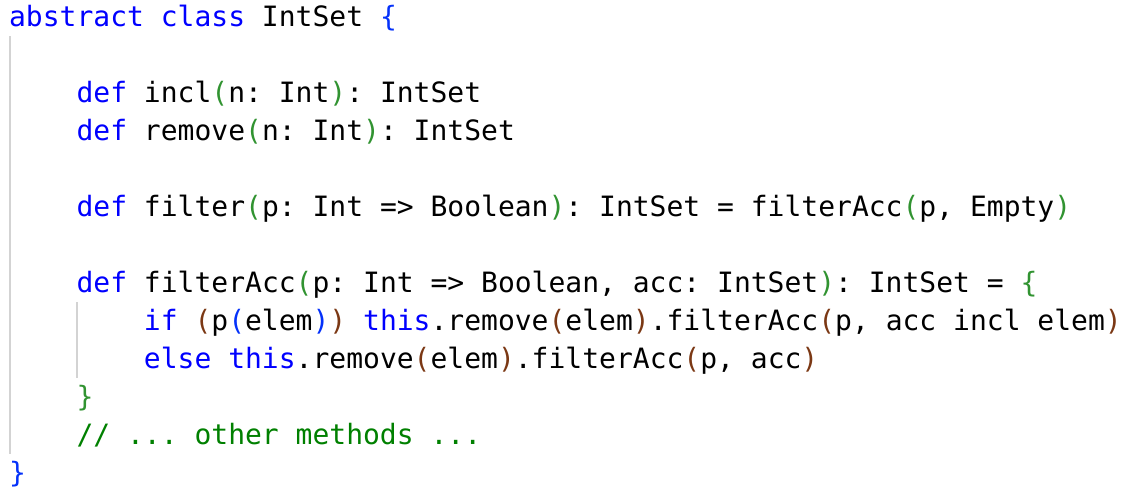
\includegraphics[scale=.3]{IntSet}

  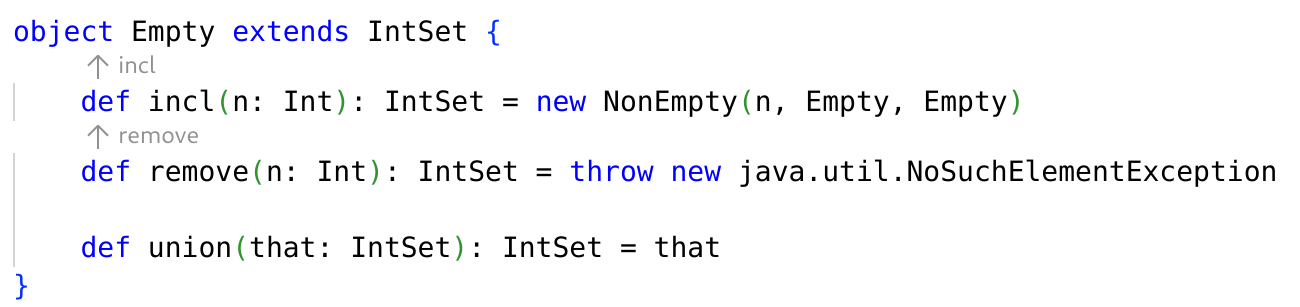
\includegraphics[scale=.3]{Empty}

  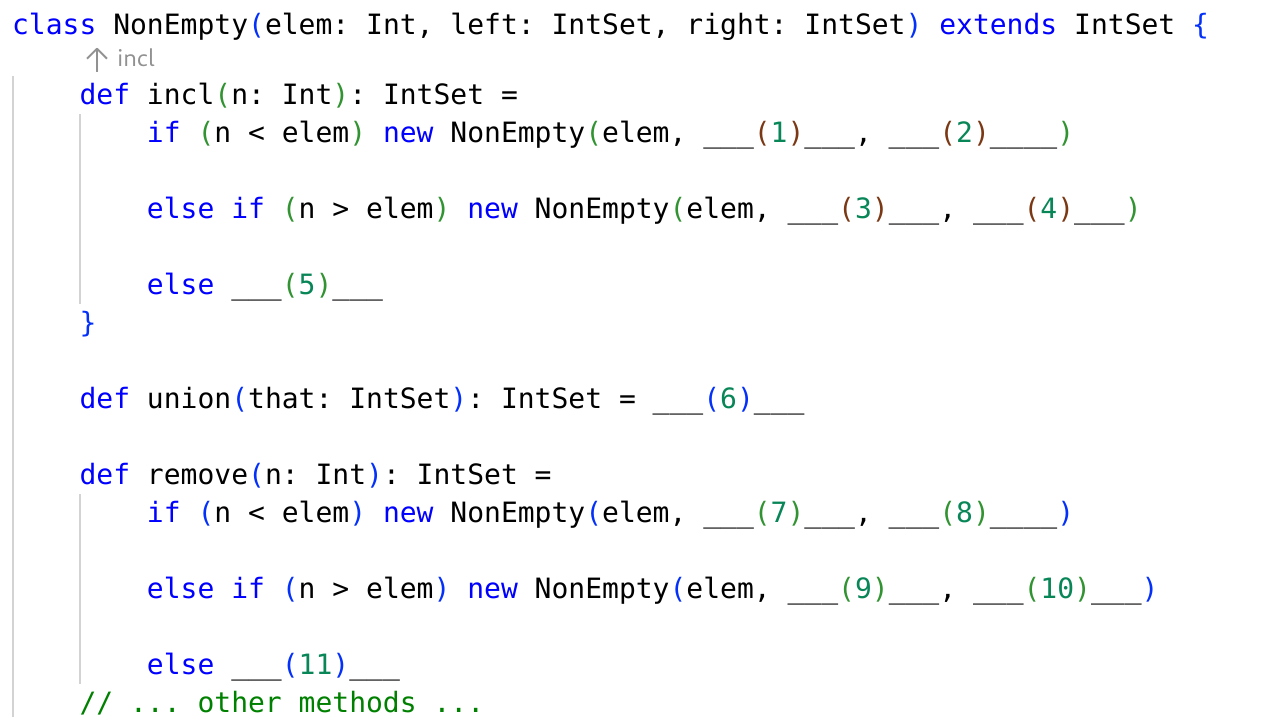
\includegraphics[scale=.3]{NonEmpty}

  \begin{parts}

    \part If \texttt{s} is a \texttt{NonEmpty IntSet} representing the set \{1, 2, 3, 4, 5\}, what does the call \texttt{s.filter(x => x < 3)} do?

    \begin{checkboxes}
      \choice It returns an \texttt{Empty IntSet}.
      \choice It returns a \texttt{NonEmpty IntSet} representing the set \{1, 2\}.
      \CorrectChoice It throws a \texttt{NoSuchElementException}.
      \choice Nothing; the function call does not terminate.
      %\choice the program does not terminate
    \end{checkboxes}

\medskip

    \part Given your answer to the last part, what can you say about the above implementation of \texttt{filterAcc}? (select two)

    \begin{checkboxes}
      \choice It is a recursive function that returns a filtered \texttt{IntSet}.
      \choice It is a non-recursive function that never terminates.
      \choice It is a recursive function that handles the base case correctly.
      \CorrectChoice It is a recursive function that does not handle the base case correctly.
      \CorrectChoice It should not be implemented in the abstract \texttt{IntSet} class.
    \end{checkboxes}


\medskip

    \part Assuming \texttt{incl(n: Int)} should return a new \texttt{IntSet} which contains all elements of \texttt{this} set, along with the the new element \texttt{n} in case it does not already exist in this set, what goes in spaces (1), (2)?

    \begin{oneparcheckboxes}
      \choice \texttt{left}, \; \texttt{right} \; \;
      \CorrectChoice \texttt{left.incl(n)}, \; \texttt{right} \; \;
      \choice \texttt{left}, \; \texttt{right.incl(n)} \\[4pt]
      \choice \texttt{left.remove(n)}, \; \texttt{right}\;\;
      \choice \texttt{left}, \; \texttt{right.remove(n)}
    \end{oneparcheckboxes}

\bigskip

    \part What goes in (3), (4)?

    \begin{oneparcheckboxes}
      \choice \texttt{left},  \; \texttt{right} \;\;
      \choice \texttt{left.incl(n)}, \; \texttt{right} \;\;
      \CorrectChoice \texttt{left}, \; \texttt{right.incl(n)} \\[4pt]
      \choice \texttt{left.remove(n)}, \; \texttt{right}\;\;
      \choice \texttt{left}, \; \texttt{right.remove(n)}
    \end{oneparcheckboxes}

\bigskip

    \part What goes in (5)?

    \begin{checkboxes}
      \CorrectChoice \texttt{this}
      \choice \texttt{this union that}
      \choice \texttt{left union right}
      \choice \texttt{(left union right) incl that}
      \choice \texttt{((left union right) union that) incl n}
    \end{checkboxes}

\bigskip

    \part Assuming \texttt{union(that: IntSet)} should return a new \texttt{IntSet} that is the union of the \texttt{IntSet}s \texttt{this}  and \texttt{that}, what goes in (6)?

    \begin{checkboxes}
      \choice \texttt{this}
      \choice \texttt{this union that}
      \choice \texttt{left union right}
      \choice \texttt{(left union right) incl that}
      \CorrectChoice \texttt{((left union right) union that) incl elem}
    \end{checkboxes}

\bigskip

    \part Assuming \texttt{remove(n: Int)} should return an \texttt{IntSet} that does not contain
\texttt{n}, but contains all other elements of \texttt{this}, what goes in (7), (8)?

    \begin{oneparcheckboxes}
      \choice \texttt{left}, \;  \texttt{right}\;\;
      \choice \texttt{left.incl(n)}, \;  \texttt{right}\;\;
      \choice \texttt{left},\;  \texttt{right.incl(n)}\\[4pt]
      \CorrectChoice \texttt{left.remove(n)}, \;\texttt{right}\;\;
      \choice \texttt{left}, \; \texttt{right.remove(n)}
    \end{oneparcheckboxes}

\bigskip

    \part What goes in (9), (10)?

    \begin{oneparcheckboxes}
      \choice \texttt{left}, \; \texttt{right}\;\;
      \choice \texttt{left.incl(n)}, \; \texttt{right}\;\;
      \choice \texttt{left}, \; \texttt{right.incl(n)}\\[4pt]
      \choice \texttt{left.remove(n)}, \; \texttt{right}\;\;
      \CorrectChoice \texttt{left},\;  \texttt{right.remove(n)}
    \end{oneparcheckboxes}

\bigskip

    \part What goes in (11)?
    \begin{checkboxes}
      \choice \texttt{this}
      \choice \texttt{this union that}
      \CorrectChoice \texttt{left union right}
      \choice \texttt{(left union right) incl that}
      \choice \texttt{((left union right) union that) incl elem}
    \end{checkboxes}


  \end{parts}

\newpage



  \question[9] \textbf{Latency and fault-tolerance}.

\medskip

  \begin{parts}
  
    \part \textit{Latency} is degradation in performance due to... (select two)

    \begin{checkboxes}
      \choice a small number of cores in the central processing unit
      \CorrectChoice slow data transfer across the network or cluster
      \CorrectChoice shuffling data between different nodes in a cluster
      \choice stack overflow caused by recursion
    \end{checkboxes}

    \bigskip

    \part Hadoop achieves fault-tolerance by...

    \begin{checkboxes}
      \choice using lazy evaluation and garbage collection.
      \CorrectChoice writing intermediate computations to disk.
      \choice keeping all data immutable and in-memory.
      \choice replaying functional transformations over the original (immutable) dataset.
    \end{checkboxes}

    \bigskip

    \part Which is \textbf{not} one of the ways Spark decreases latency while remaining fault-tolerant?

    \begin{checkboxes}
      \choice using ideas from functional programming.
      \CorrectChoice using ideas from imperative programming; e.g., mutation and side effects.
      \choice keeping all data immutable and in-memory.
      \choice replaying functional transformations over the original (immutable) dataset.
    \end{checkboxes}

  \end{parts}

  \bigskip

  \question[12] \textbf{Transformations and actions}.

  \medskip

  \begin{parts}
  
    \part A \textbf{transformation} on an RDD... (select two)

    \begin{checkboxes}
      \CorrectChoice does not immediately compute a result.
      \choice immediately computes and returns a result.
      \CorrectChoice is lazily evaluated.
      \choice is eagerly evaluated.
    \end{checkboxes}

    \bigskip
    \part An \textbf{action} on an RDD... (select two)

    \begin{checkboxes}
      \choice does not immediately compute a result.
      \CorrectChoice immediately computes and returns a result.
      \choice is lazily evaluated.
      \CorrectChoice is eagerly evaluated.
    \end{checkboxes}

    \bigskip

    \part After performing a series of transformations on an \texttt{RDD}, which of the following methods would ensure that Spark actually carries out the transformations.

    \begin{oneparcheckboxes}
      \choice \texttt{mapValues()}
      \CorrectChoice \texttt{collect()}
      \choice \texttt{groupBy()}
      \choice none of these
    \end{oneparcheckboxes}

    \bigskip

    \part After performing a series of transformations on an \texttt{RDD}, which of the following methods could you use to make sure those transformations are not repeated unnecessarily?

    \begin{oneparcheckboxes}
      \choice \texttt{save()}
      \CorrectChoice \texttt{persist()}
      \choice \texttt{collect()}
      \choice \texttt{parallelize()}
    \end{oneparcheckboxes}

    \newpage

    \part Why does the \texttt{RDD} class have no \texttt{foldLeft} method?

    \begin{checkboxes}
      \choice \texttt{foldLeft} is not stack-safe.
      \choice \texttt{foldLeft} is not fault-tolerant.
      \choice \texttt{foldLeft} only works on \texttt{PairRDD}s.
      \CorrectChoice \texttt{foldLeft} is not parallelizable.
      \choice It's not true; the RDD class \textit{does} have a \texttt{foldLeft} method.
    \end{checkboxes}

    \bigskip

    \part Which method of the \texttt{RDD} class has the same effect as \texttt{foldLeft} and overcomes limitations of the latter?

  \begin{oneparcheckboxes}
    \CorrectChoice \texttt{aggregate}
      \choice \texttt{foldRight}
      \choice \texttt{join}
    \choice \texttt{leftOuterJoin}
    \choice \texttt{collect}
  \end{oneparcheckboxes}

  \end{parts}



\end{questions}


\end{document}


